\documentclass{article}
\usepackage{amsmath}
\usepackage{xcolor}
\usepackage{gensymb}
\usepackage{ragged2e}
\usepackage{graphicx}
\usepackage{gensymb}
\usepackage{mathtools}
\newcommand{\mydet}[1]{\ensuremath{\begin{vmatrix}#1\end{vmatrix}}}
\providecommand{\brak}[1]{\ensuremath{\left(#1\right)}}
\providecommand{\norm}[1]{\left\lVert#1\right\rVert}
\newcommand{\solution}{\noindent \textbf{Solution: }}
\newcommand{\myvec}[1]{\ensuremath{\begin{pmatrix}#1\end{pmatrix}}}
\let\vec\mathbf
\begin{document}
\begin{center}
        \textbf\large{CHAPTER-11 \\ TRIANGLES}
\end{center}
\section{Exercise 11.2}
Q2.Construct a triangle $ABC$ in which $BC=7cm$,$\angle{B}=45^0$ and $AB-AC=3.5cm$. \\
\textbf{Solution:}\\
Let $\vec{A}$,$\vec{B}$ and $\vec{C}$ are the vertices of the triangle with coordinates.
Given $BC=8cm$.So the coordinates of vertices $\vec{B}$,$\vec{C}$ are:
\begin{center}
{
$\vec{B}$ =$\begin{pmatrix}
0 \\
0 
\end{pmatrix}$ 
\vspace{1mm}
$\vec{C}$=$\begin{pmatrix}
8 \\
0
\end{pmatrix}$ 
\vspace{1mm}
}
\end{center}
Also given $\angle{B}=45^0$,so by finding the coordinates of the other side we can form a required triangle. \\
 \vspace{2mm}
 The input parameters for this construction are
 \begin{table}[h]
	  \centering
	  \begin{tabular}{|c|c|c|}
  \hline
  \textbf{Symbol}&\textbf{Value}&\textbf{Description}\\
  \hline
  a & 8cm & BC\\
  \hline
  $\theta$ & $45^0$ & $\angle{BC}$ in $\Delta$ABC \\
  \hline
	k & 3.5 & AB-AC i.e(c-b)\\
  \hline
\end{tabular}

	  \caption{Parameters}
	  \label{tab:Table1}
\end{table}


\raggedright\textbf{Caluclating Other Coordinate: } \\
  \raggedright Let $\vec{A}$ = b$\times$
  $\begin{pmatrix} 
 \cos \theta\\
  \sin\theta \\
\end{pmatrix}$ \\
\raggedright Using the Cosine formula in  $\Delta$ABC, \\ \vspace{3mm}
\begin{equation}
{b}^2 = {a}^2 + {c}^2 - 2accos\vec{B}
\end{equation}
\begin{equation}
(b+c)(b-c) = {a}^2- 2accos\vec{B}
\end{equation}
Given
\begin{equation}
        c-b=k
	\end{equation}
  \begin{equation}
        b-c=-k
 \end{equation}\\
Upon Simplifaction we get:- \\
\begin{equation}
(b+c)(-k) = {a}^2- 2accos\vec{B}
\end{equation}
\begin{equation}
-kc-kb+2accos\vec{B}= {a}^2
\end{equation}
\begin{equation}
-kb-c(k-2acos\vec{B})= {a}^2
\end{equation} \\
\pagebreak
     From equations (4) and (7) , we obtain the matrix equation:- \\ \vspace{3mm}
     \begin{equation}
        \begin{pmatrix}
	   1 & -1  \\	
	  -k & -k+2acos\vec{B}    \\
        \end{pmatrix}
        \begin{pmatrix}
            b \\
            c \\
        \end{pmatrix}
           =
           \begin{pmatrix}
            -k\\
            a^2\\
        \end{pmatrix}   
\end{equation}	     
        \vspace{5mm}           
   \\  
   \begin{equation}
    \begin{pmatrix}
	    1 & -1 \\
           -3.5 & -3.5+2(8)cos45^0 \\
            
        \end{pmatrix}
        \begin{pmatrix}
            b \\
            c \\
        \end{pmatrix}
           =
           \begin{pmatrix}
           -3.5\\
            64\\
        \end{pmatrix}
	\end{equation}
        \vspace{5mm}           
   \\  
   The augmented matrix for the above matrix equation is 
\vspace{3mm}
\begin{equation}
\begin{pmatrix}
   1 & -1 & \vrule & -3.5 \\
  -3.5 & 7.81 & \vrule & 64
    \end{pmatrix}  
    \end{equation}
   \vspace{5mm}
    Reducing to echelon form:-
   \\
   \begin{center}
    $\begin{pmatrix}
	    \myvec{ 1 &-1  & -3.5 \vspace{5mm} \\ 0 & \frac{4.31}{3.5} & \frac{51.75}{3.5}}
	    \xleftarrow{R_2 \leftarrow \frac{1}{3.5}R_2+R_1}
    \end{pmatrix}$
	   \\
   \end{center}
  \vspace{5mm}
  \begin{center}
   $\begin{pmatrix}
	   \myvec{1 &-1  & -3.5 \vspace{5mm} \\ 0 & 1 & \frac{51.75}{4.31}}
	   \xleftarrow{R_2 \leftarrow \frac{3.5}{4.31}R_2}
    \end{pmatrix}$
  \\
	  \end{center}
  \vspace{5mm}
  \begin{center}
  $\begin{pmatrix}
	  \myvec{1 & 0 & \frac{36.67}{4.31} \vspace{5mm}\\ 0 & 1 & \frac{51.75}{4.31}}
    \xleftarrow{R1 \leftarrow R_1+R_2}
    \end{pmatrix}$
  \\
	  \end{center}
  \vspace{5mm}
  Reduced Echelon Form: 
  \begin{center}
  $\begin{pmatrix}
	  1 & 0 & 8.5 \\ 0 & 1 & 12
    \end{pmatrix}$
    \\
	  \end{center}
    \vspace{5mm}
      $\begin{pmatrix}
            b\\
            c\\
        \end{pmatrix}$
            =
            $\begin{pmatrix}
            8.5\\
            12\\
        \end{pmatrix}$
        \vspace{3mm}
	\pagebreak
   \\  The vertices of $\Delta$ ABC are \\ \vspace{3mm}
     \raggedright \textbf{A} = 8.5$\begin{pmatrix}
                 cos 45 \\ 
                 sin 45 \\
              \end{pmatrix}$
              =$\begin{pmatrix}
                 6.01 \\
                 6.01 \\
                 \end{pmatrix}$
                 \vspace{5mm}
              \\ \raggedright  \textbf{B} = $\begin{pmatrix}
                 0\\
                 0\\
              \end{pmatrix}$
              \vspace{5mm}
             \\ \raggedright  \textbf{C} = $\begin{pmatrix}
                  8\\
                  0\\
              \end{pmatrix}$
              \\
	      \vspace{5mm}
\textbf{Construction:}\\
\begin{figure}[h]
 \begin{center}
	 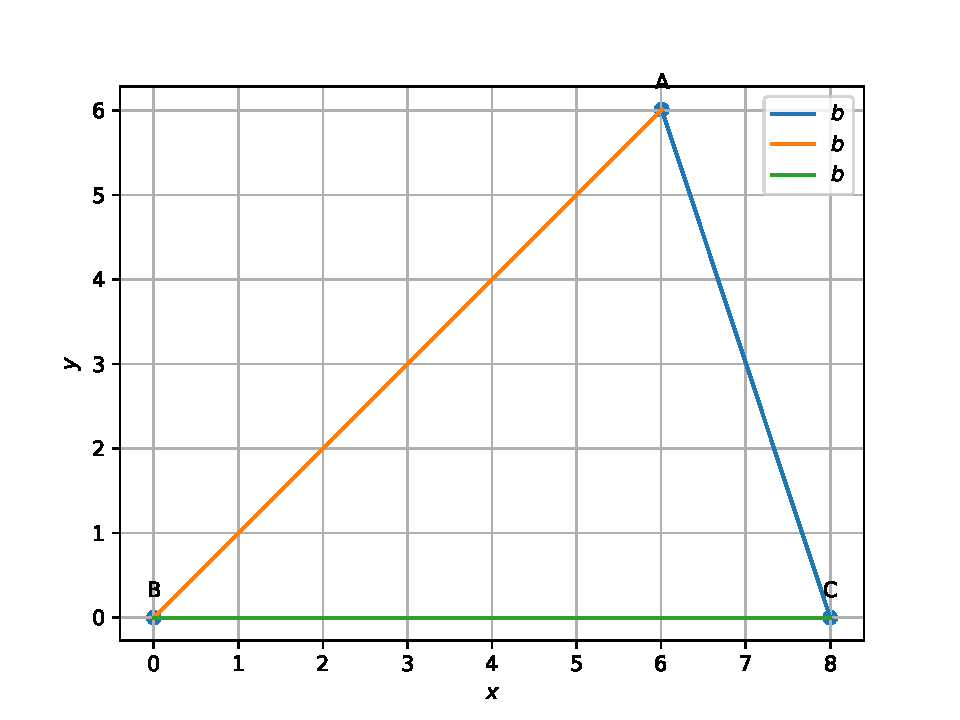
\includegraphics[width=0.5\textwidth]{figs/triangle.pdf}
 \end{center}
 \caption{Triangle ABC}
 \label{fig:Fig1}
\end{figure}	
\end{document}
